\documentclass[usenames,dvipsnames,11pt,pdf,utf8,russian,aspectratio=43]{beamer}
\usepackage{cmap}
\usepackage[T2A]{fontenc}
\usepackage[english,russian]{babel}
\usepackage{subfig}
\usepackage{color}
\usepackage{multicol}
\usepackage{appendixnumberbeamer}
\usepackage{multicol}
\usepackage{tikz}
\usepackage{mathbbol}
\usepackage{amssymb}             % AMS Math

\DeclareSymbolFontAlphabet{\mathbb}{AMSb}%
\DeclareSymbolFontAlphabet{\amsmathbb}{bbold}%


\usetikzlibrary{arrows,automata}
\usetikzlibrary{positioning}



\DeclareMathOperator*{\argmin}{arg\,min}

\DeclareMathOperator*{\argmax}{arg\,max}
%
% Choose how your presentation looks.
%
% For more themes, color themes and font themes, see:
% http://deic.uab.es/~iblanes/beamer_gallery/index_by_theme.html
%
\mode<presentation>
{
  \usetheme{Boadilla}      % or try Darmstadt, Madrid, Warsaw, ...
  \usecolortheme{seagull} % or try albatross, beaver, crane, ..

  \usefonttheme{structurebold}  % or try serif, structurebold, ...
  \setbeamertemplate{navigation symbols}{}
  \setbeamertemplate{caption}[numbered]
} 

\captionsetup[subfloat]{labelformat=empty}
\title[Выбор структуры модели]{Байесовский выбор\\ субоптимальной структуры\\ модели глубокого обучения}
\author{О.\,Ю.\,Бахтеев}


\institute[]{Диссертация на соискание ученой степени\\
кандидата физико-математических наук\\05.13.17 --- Теоретические основы информатики\\Научный руководитель: д.ф.-м.н. В.В. Стрижов\\}     
%\institute[МФТИ]{Московский Физико-Технический Институт (Государственный Университет)}
\date[2019]{Московский физико-технический институт\\16 июня 2019 г.}
\begin{document}

\begin{frame}
  \titlepage
\end{frame}



\begin{frame}{Выбор  структуры модели глубокого обучения}
\footnotesize
\textbf{Цель работы:}\\
Предложить метод выбора структуры модели глубокого обучения.\\
\textbf{Задачи:}
\begin{enumerate}
\item Предложить критерии оптимальной и субоптимальной сложности модели глубокого обучения.
\item Предложить алгоритм построения модели субоптимальной сложности и оптимизации параметров.
\end{enumerate}
\textbf{Основные проблемы:}
\begin{enumerate}
\item Большое число параметров и гиперпараметров.
\item Многоэкстремальность и невыпуклость задачи оптимизации параметров и гиперпараметров модели.
\item Высокая вычислительная сложность оптимизации.
\end{enumerate}
\textbf{Методы исследования.}\\ 
Используются методы вариационного байесовского вывода. Рассматриваются графовое представление нейронной сети. Для получения вариационных оценок правдоподобия модели используется метод, основанный на градиентном спуске. В качестве метода получения модели субоптимальной сложности используется метод автоматического определения релевантности параметров с использоваением градиентных методов оптимизации гиперпараметров.
\end{frame}



\begin{frame}    
                                                                                                                        
\frametitle{Проблема выбора оптимальной структуры модели глубокого обучения}                                                                                                          
Правдоподобие моделей с избыточным числом параметров не меняется при их удалении.                                                       
\begin{figure}[h]                                                                                                                               
\centering                                                                                                                                      
\subfloat[Избыточность параметров модели]{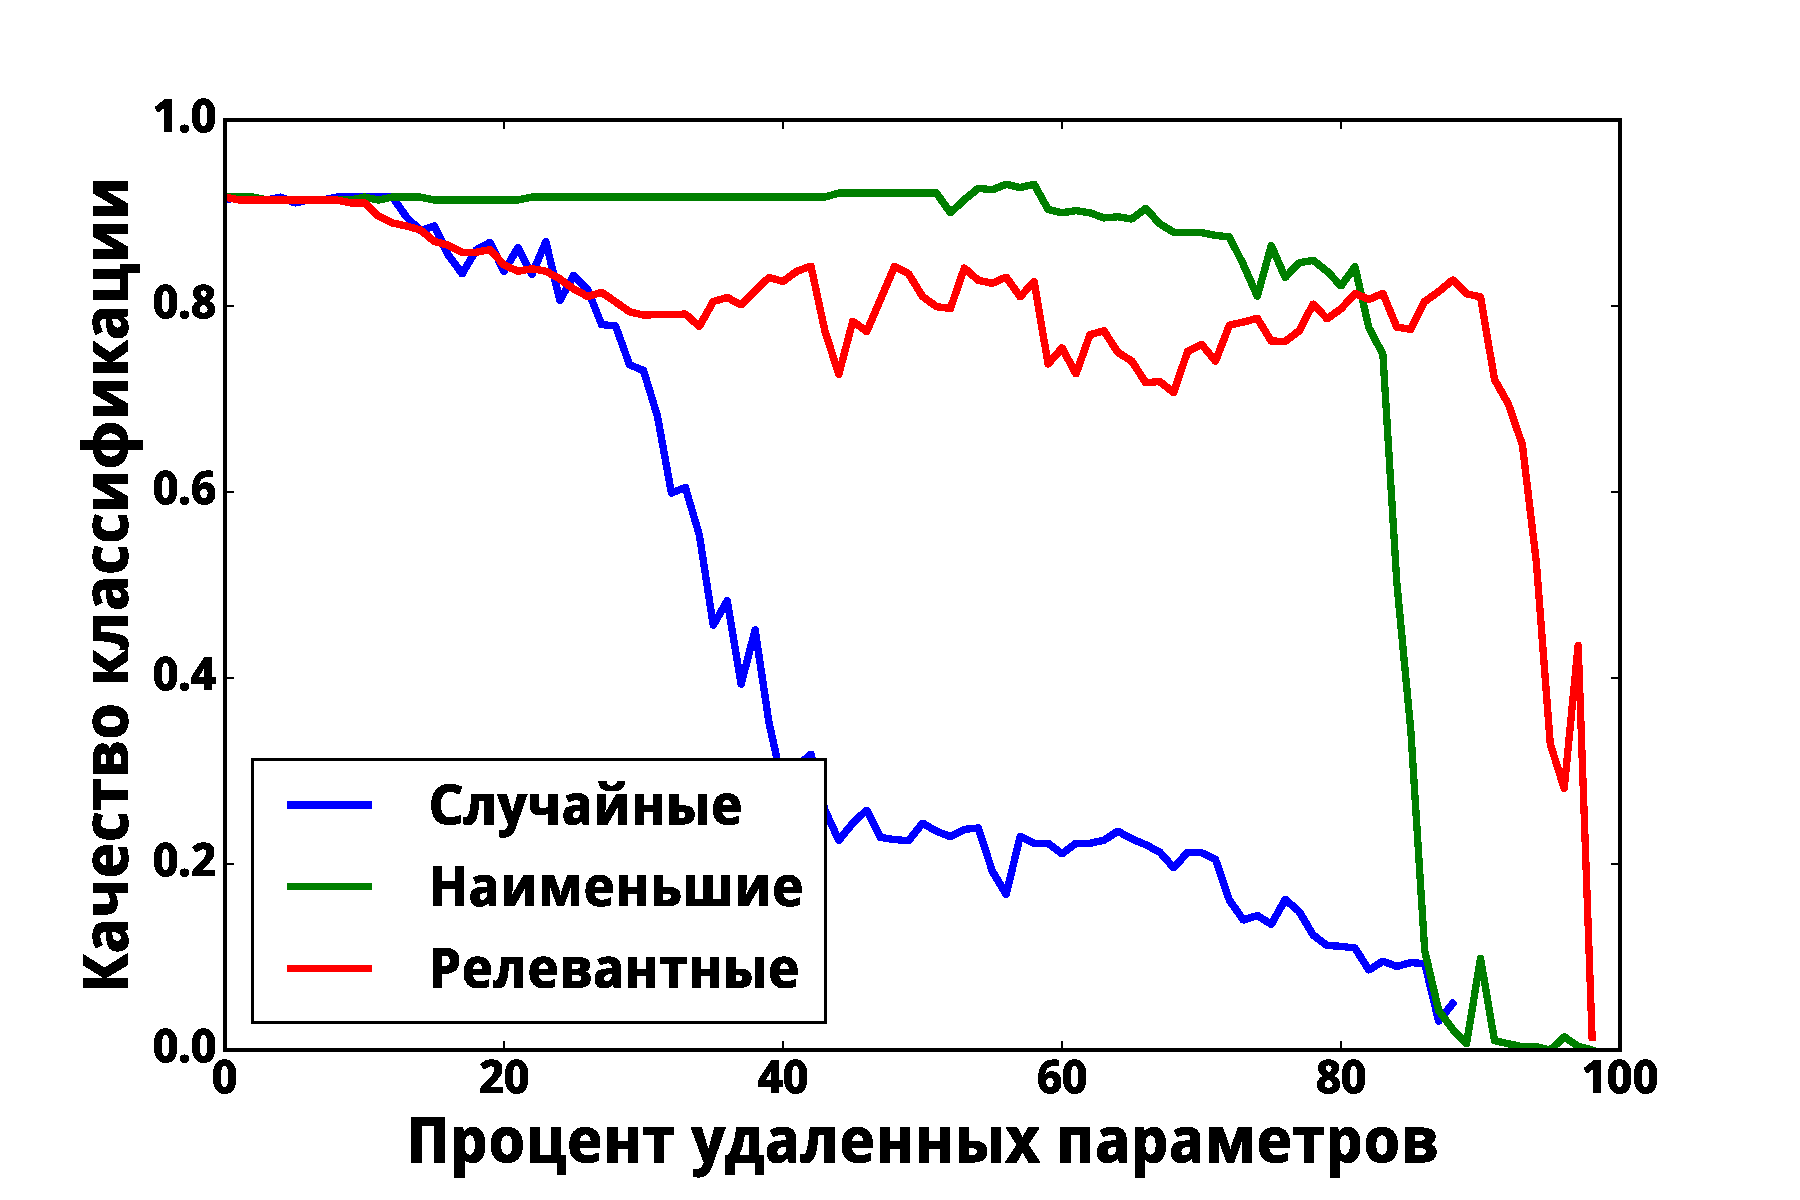
\includegraphics[width=0.5\textwidth]{./slide_plots/pruning.pdf}}                                          
\subfloat[Неустойчивость модели]{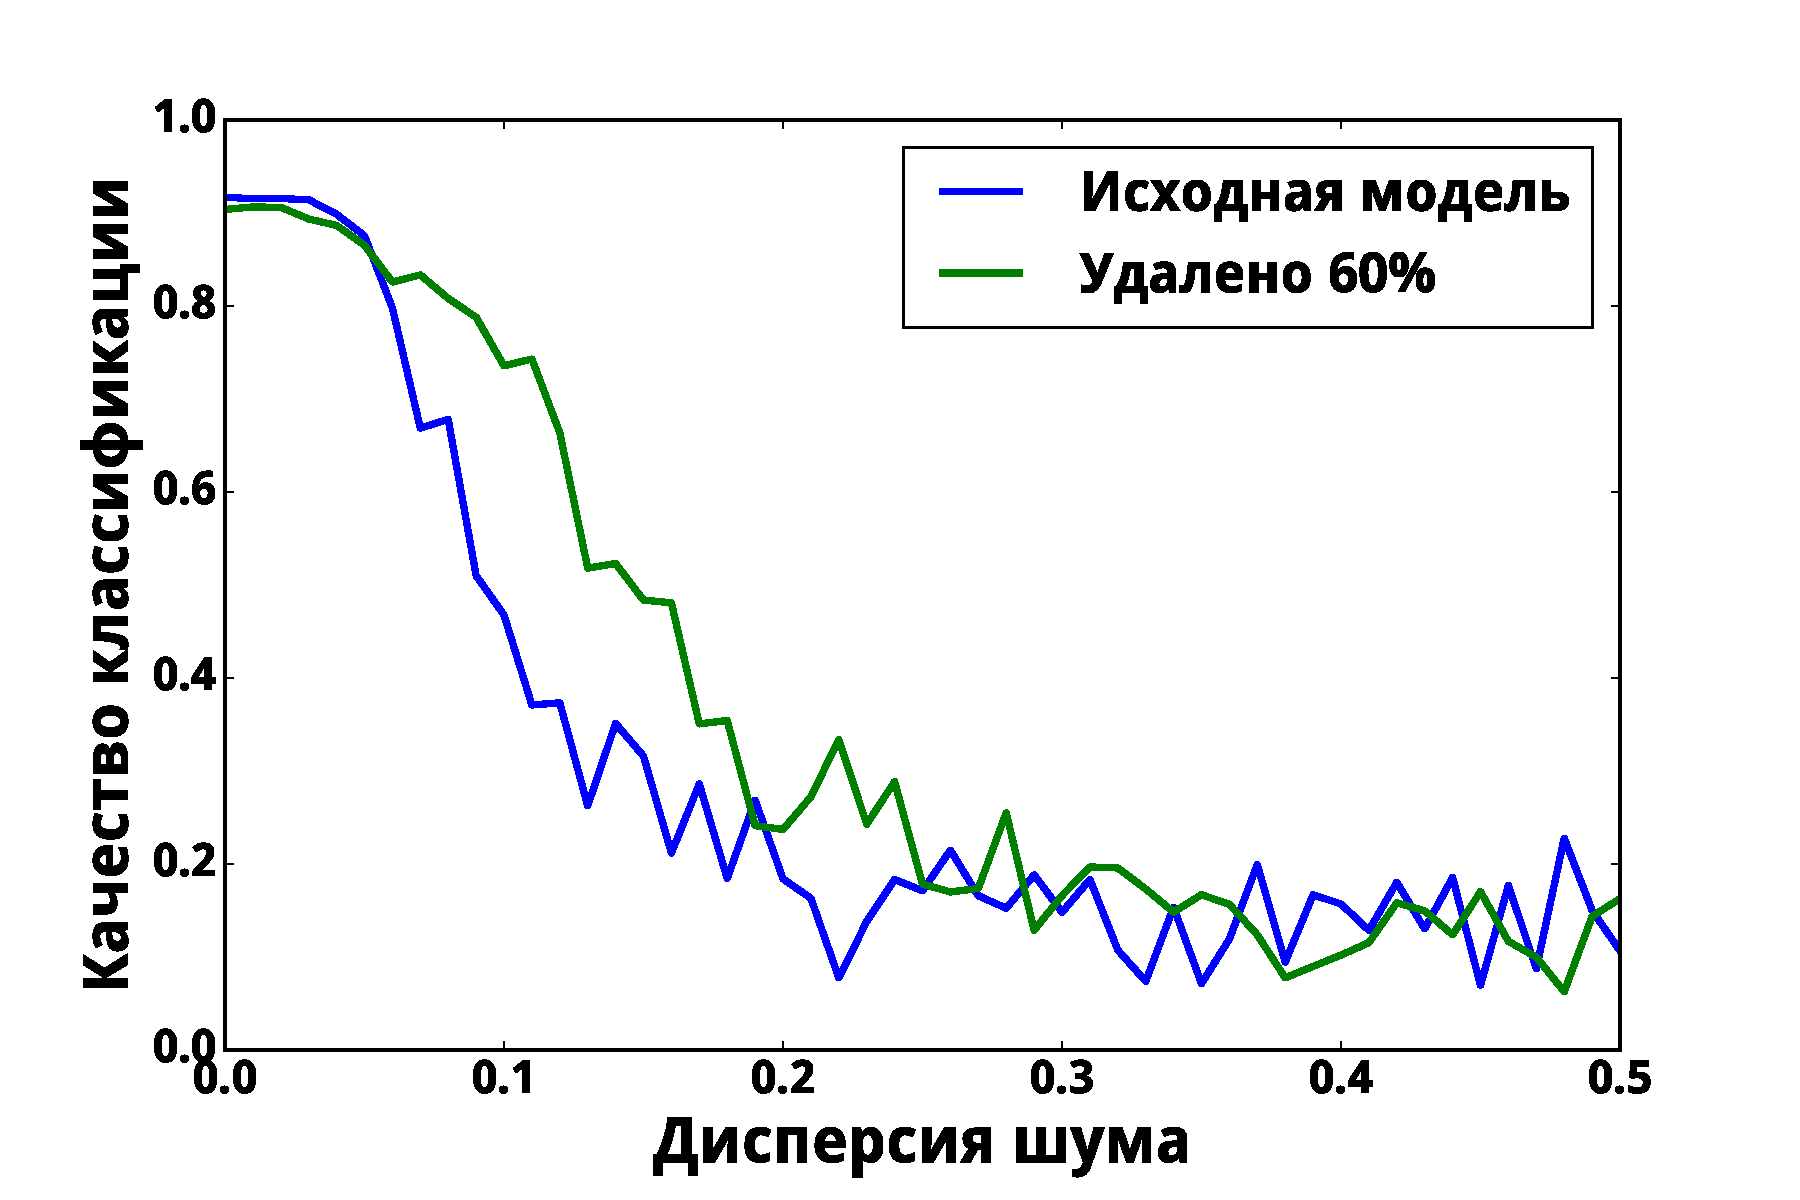
\includegraphics[width=0.5\textwidth]{./slide_plots/noise.pdf}}                                                     
\end{figure}                                                                                                   
\textcolor{gray}{Глубокое обучение предполагает оптимизацию моделей с заведомо избыточной сложностью.}  

                                                                                                                                             
\end{frame}    

\begin{frame}{Выбор структуры: двуслойная нейросеть}
\small
\textbf{Структурные параметры:} $\boldsymbol{\Gamma} = [\boldsymbol{\gamma}^{0,1}, {\boldsymbol{\gamma}^{1,2}}].$

\[
    \mathbf{f}(\mathbf{x}) = \textbf{softmax}\left(\mathbf{W}^{1,2}_0\text{T}{\mathbf{f}_1}(\mathbf{x})\right), \quad f(\mathbf{x}): \mathbb{R}^n \to [0,1]^{|\mathbb{Y}|}, \quad \mathbf{x} \in \mathbb{R}^n.
\]
\[
\mathbf{f}_1(\mathbf{x}) = {\gamma}^{0,1}_{0}\mathbf{g}^{0,1}_{0}(\mathbf{x}) + {\gamma}^{0,1}_{1}\mathbf{g}^{0,1}_{1}(\mathbf{x})
\]
где $\mathbf{W} = [\mathbf{W}^{0,1}_0, \mathbf{W}^{0,1}_1, \mathbf{W}^{1,2}_0]^{\text{T}}$ --- матрицы параметров, $\{\mathbf{g}^{0}_{0,1},\mathbf{g}^{1}_{0,1},{\mathbf{g}^{0}_{1,2}\}}$ --- обобщенно-линейные функции скрытых слоев нейросети.

\begin{tikzpicture}[node distance=0.5cm, auto]
  %\tikzstyle{every state}=[fill=red,draw=none,text=white]

  \node (f0)  at (1,6)                  {$\mathbf{f}_0(\mathbf{x}) = \mathbf{x}$};
  %\node (g11) at (6,3)                    {$\mathbf{g}^{1,1}(\mathbf{x})$};% = \text{Conv}(\mathbf{x}, 3, 32, 1)$};
  %\node (g12)  at (6,9)                   {$\mathbf{g}^{1,2}(\mathbf{x})$};% = \text{Conv}(\mathbf{x}, 4, 32, 1)$};
  \node (f1)  at (7,6)                 {$\mathbf{f}_1(\mathbf{x})$};% = \gamma^{1,1}\mathbf{g}^{1,1}(\mathbf{x}) +  \gamma^{1,2}\mathbf{g}^{1,2}(\mathbf{x})$};
  %\node (g21) at (12,6)                   {$\mathbf{g}^{2,1}(\mathbf{x})$};% = \boldsymbol{\sigma}(\mathbf{w}^{2,1}\mathbf{x})$};
  \node (f2)  at (12,6)                   {$\mathbf{f}_2(\mathbf{x})$};% = \gamma^{2,1}\mathbf{g}^{2,1}(\mathbf{x})$};
  \path[->]  (f0) edge [bend left=50] node {$\gamma^{0,1}_0\mathbf{g}^{0,1}_0(\mathbf{x}) = \gamma^{0,1}_0\boldsymbol{\sigma}(\mathbf{W}^{0,1}_0\mathbf{x})$}(f1);
  \path[->] (f0)  edge[bend right=50] node[below] {$\gamma^{0,1}_1\mathbf{g}^{0,1}_1(\mathbf{x}) = \gamma^{0,1}_1\boldsymbol{\sigma}(\mathbf{W}^{0,1}_1\mathbf{x})$}(f1);
  \path[->] (f1)  edge node {$\gamma^{1,2}_0\mathbf{g}^{1,2}_0(\mathbf{x}) = \gamma^{1,2}_0\textbf{softmax}(\mathbf{W}^{1,2}_0\mathbf{x})$}(f2);       
  \draw[->] (f1) to (f2);
 
\end{tikzpicture}

\end{frame}


\begin{frame}{Графовое представление модели глубокого обучения}
\footnotesize
\begin{block}{Определение}
Пусть:
\begin{enumerate}
\item задан ациклический граф $(V,E)$;
\item для каждого ребра $(j,k) \in E$ определен вектор базовых функций  мощности $K^{j,k}$: $\mathbf{g}^{j,k} = [\mathbf{g}^{j,k}_0, \dots, \mathbf{g}^{j,k}_{K^{j,k}}]$;
\item для каждой вершины $v \in V$ определена функция агрегации $\textbf{agg}_v$.
\end{enumerate}
Граф $(V, E)$ в совокупности со множестом векторов базовых функций $\{\mathbf{g}^{j,k}, (j,k) \in E\}$ и множеством функций агрегаций $\{ \textbf{agg}_v, {v \in V}\}$ задает \textit{параметрическое семейство моделей} $\mathfrak{F}$, если функция $\mathbf{f} = \mathbf{f}_{|V|-1}$, задаваемая по правилу 
\begin{equation}
\label{eq:modelfam}
    \mathbf{f}_{v}(\mathbf{w}, \mathbf{x}) = \textbf{agg}_{v}\left(\{ \langle \boldsymbol{\gamma}^{j,k}, \mathbf{g}^{j,k} \rangle \left(\mathbf{f}_j(\mathbf{x})\right)| j \in \text{Adj}(v_k)\}\right), v \in \{1,\dots,|V|-1\}, \quad \mathbf{f}_0(\mathbf{x}) = \mathbf{x}
\end{equation}
является дифференцируемой  по параметрам $\mathbf{w}$ функцией из признакового пространства $\mathbb{X}$ в пространство меток $\mathbb{Y}$ при значениях векторов, $\boldsymbol{\gamma}^{j,k} \in [0,1]^{K^{j,k}}$.

\end{block}
\end{frame}

      

\begin{frame}{Ограничения на структурные параметры}
Примеры ограничений для одного структурного параметра $\boldsymbol{\gamma}, |\boldsymbol{\gamma}| = 3$.
\begin{figure}
 \begin{minipage}[t]{.45\textwidth}
        \centering
%1 limit
\begin{tikzpicture}[%
x={(1.5cm,0cm)},
y={(0cm,1.5cm)},
z={({0.5*cos(45)},{0.5*sin(45)})},
]

\coordinate (A) at (0,0,0); 
\coordinate (B) at (1,0,0) ;
\coordinate (C) at (1,1,0); 
\coordinate (D) at (0,1,0); 
\coordinate (E) at (0,0,1); 
\coordinate (F) at (1,0,1); 
\coordinate (G) at (1,1,1); 
\coordinate (H) at (0,1,1   );

%Ecken
\node[circle,scale=0.5,fill=black,draw=black](Ap) at (0,0,0){};
\node[circle,scale=0.5,fill=black,draw=black](Bp) at (1,0,0){};
\node[circle,scale=0.5,fill=black,draw=black](Cp) at (1,1,0){};
\node[circle,scale=0.5,fill=black,draw=black](Dp) at (0,1,0){};
\node[circle,scale=0.5,fill=black,draw=black](Ep) at (0,0,1){};
\node[circle,scale=0.5,fill=black,draw=black](Fp) at (1,0,1){};
\node[circle,scale=0.5,fill=black,draw=black](Gp) at (1,1,1){};
\node[circle,scale=0.5,fill=black,draw=black](Hp) at (0,1,1){};
\node[left= 1pt of A]{[0,0,0]};
\node[right= 1pt of B]{[1,0,0]};
\node[right= 1pt of C]{[1,1,0]};
\node[left= 1pt of D]{[0,1,0]};
\node[left= 1pt of E]{[0,0,1]};
\node[right= 1pt of F]{[1,0,1]};
\node[right= 1pt of G]{[1,1,1]};
\node[left= 1pt of H]{[0,1,1]};

%Kanten
\draw[] (A)
-- (B)  node[midway, below]{}
-- (C)      node[midway, right]{}
-- (D)  node[midway, above]{}
-- (A)  node[midway, left]{};
\draw[] (B) -- (F) -- (G) -- (C);
\draw[] (G) -- (H) -- (D);
\draw[densely dashed] (A) -- (E) -- (F);
\draw[densely dashed] (E) -- (H);

\end{tikzpicture}
\caption*{Структурный параметр лежит на вершинах куба}
\end{minipage}
\hfill
 \begin{minipage}[t]{.45\textwidth}
        \centering

%2 limit
\begin{tikzpicture}[%
x={(1.5cm,0cm)},
y={(0cm,1.5cm)},
z={({0.5*cos(45)},{0.5*sin(45)})},
]

\coordinate (A) at (0,0,0); 
\coordinate (B) at (1,0,0) ;
\coordinate (C) at (1,1,0); 
\coordinate (D) at (0,1,0); 
\coordinate (E) at (0,0,1); 
\coordinate (F) at (1,0,1); 
\coordinate (G) at (1,1,1); 
\coordinate (H) at (0,1,1   );

%Ecken
\node[left= 1pt of A]{[0,0,0]};
\node[right= 1pt of B]{[1,0,0]};
\node[right= 1pt of C]{};
\node[left= 1pt of D]{[0,1,0]};
\node[left= 1pt of E]{};
\node[right= 1pt of F]{[1,0,1]};
\node[right= 1pt of G]{[1,1,1]};
\node[left= 1pt of H]{[0,1,1]};

%Kanten
\draw[fill=gray] (A)
-- (B)  node[midway, below]{}
-- (C)      node[midway, right]{}
-- (D)  node[midway, above]{}
-- (A)  node[midway, left]{};
\draw[fill=gray] (B) -- (F) -- (G) -- (C);
\draw[fill=gray] (G) -- (H) -- (D);
\draw[fill=gray] (A) -- (E) -- (F);
\draw[fill=gray] (E) -- (H);
\draw[fill=gray] (D) -- (H) -- (G) -- (C);
\end{tikzpicture}
\caption*{Структурный параметр лежит внутри куба}
\end{minipage}
\hfill
 \begin{minipage}[t]{.45\textwidth}
        \centering
%3 limit
\begin{tikzpicture}[%
x={(1.5cm,0cm)},
y={(0cm,1.5cm)},
z={({0.5*cos(45)},{0.5*sin(45)})},
]

\coordinate (A) at (0,0,0); 
\coordinate (B) at (1,0,0) ;
\coordinate (C) at (1,1,0); 
\coordinate (D) at (0,1,0); 
\coordinate (E) at (0,0,1); 
\coordinate (F) at (1,0,1); 
\coordinate (G) at (1,1,1); 
\coordinate (H) at (0,1,1   );

%Ecken
\node[circle,scale=0.5,fill=black,draw=black](Bp) at (1,0,0){};
\node[circle,scale=0.5,fill=black,draw=black](Dp) at (0,1,0){};
\node[circle,scale=0.5,fill=black,draw=black](Ep) at (0,0,1){};
\node[left= 1pt of A]{};
\node[right= 1pt of B]{[1,0,0]};
\node[right= 1pt of C]{};
\node[left= 1pt of D]{[0,1,0]};
\node[left= 1pt of E]{[0,0,1]};
\node[right= 1pt of F]{};
\node[right= 1pt of G]{};
\node[left= 1pt of H]{};

%Kanten
\draw[] (A)
-- (B)  node[midway, below]{}
-- (C)      node[midway, right]{}
-- (D)  node[midway, above]{}
-- (A)  node[midway, left]{};
\draw[] (B) -- (F) -- (G) -- (C);
\draw[] (G) -- (H) -- (D);
\draw[densely dashed] (A) -- (E) -- (F);
\draw[densely dashed] (E) -- (H);

\end{tikzpicture}
\caption*{Структурный параметр лежит на вершинах симплекса}
\end{minipage}
\hfill
 \begin{minipage}[t]{.45\textwidth}
        \centering
%4 limit
\begin{tikzpicture}[%
x={(1.5cm,0cm)},
y={(0cm,1.5cm)},
z={({0.5*cos(45)},{0.5*sin(45)})},
]

\coordinate (A) at (0,0,0); 
\coordinate (B) at (1,0,0) ;
\coordinate (C) at (1,1,0); 
\coordinate (D) at (0,1,0); 
\coordinate (E) at (0,0,1); 
\coordinate (F) at (1,0,1); 
\coordinate (G) at (1,1,1); 
\coordinate (H) at (0,1,1   );

%Ecken
\node[left= 1pt of A]{};
\node[right= 1pt of B]{[1,0,0]};
\node[right= 1pt of C]{};
\node[left= 1pt of D]{[0,1,0]};
\node[left= 1pt of E]{[0,0,1]};
\node[right= 1pt of F]{};
\node[right= 1pt of G]{};
\node[left= 1pt of H]{};

%Kanten
\draw[] (A)
-- (B)  node[midway, below]{}
-- (C)      node[midway, right]{}
-- (D)  node[midway, above]{}
-- (A)  node[midway, left]{};
\draw[] (B) -- (F) -- (G) -- (C);
\draw[] (G) -- (H) -- (D);
\draw[densely dashed] (A) -- (E) -- (F);
\draw[densely dashed] (E) -- (H);
\draw[fill=gray] (B) -- (D) -- (E);


\end{tikzpicture}
\caption*{Структурный параметр лежит внутри симплекса}
\end{minipage}

\end{figure}

\end{frame}






\begin{frame}{Априорное распределение параметров}
\footnotesize   
\begin{columns}
\begin{column}{0.6\textwidth}
   \begin{block}{Определение}
\textit{Априорным распределением} параметров $\mathbf{W}$ и структуры  $\boldsymbol{\Gamma}$ модели $\mathbf{f}$ назовем вероятностное распределение
$
    p(\mathbf{W}, \boldsymbol{\Gamma}|\mathbf{h}): \mathbb{W} \times \amsmathbb{\Gamma} \times \mathbb{H} \to \mathbb{R}^{+}, 
$
где $\mathbb{W}$ --- множество значений параметров модели, $\amsmathbb{\Gamma}$ --- множество значений структуры модели.
\end{block}

\end{column}
\begin{column}{0.4\textwidth}  %%<--- here
    \begin{center}
     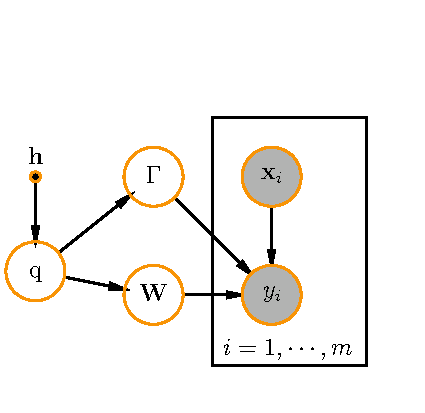
\includegraphics[width=\textwidth]{plate.pdf}
     \end{center}
\end{column}
\end{columns}
\vspace*{-0.5cm}
\begin{block}{}
\textit{Гиперпараметрами} $\mathbf{h}\in \mathbb{H}$ модели  назовем параметры распределения $p(\mathbf{w}, \boldsymbol{\Gamma}|\mathbf{h})$ (параметры распределения параметров модели $\mathbf{f}$).
\end{block}

\begin{block}{}
\textit{Вариационными параметрами} модели $\boldsymbol{\theta} \in \mathbb{R}^u$ назовем параметры распределения $q$, приближающие апостериорное распределение параметров и структыр:
\[
    q \approx p(\mathbf{W}, \boldsymbol{\Gamma}|\mathbf{X}, \mathbf{y}, \mathbf{h}) = \frac{p(\mathbf{y}|\mathbf{X},\mathbf{W},\boldsymbol{\Gamma}, \mathbf{h})p(\mathbf{W}, \boldsymbol{\Gamma}|\mathbf{h})}{\int\int_{\mathbf{W}', \boldsymbol{\Gamma'}}p(\mathbf{y}|\mathbf{X},\mathbf{W}',\boldsymbol{\Gamma}', \mathbf{h})p(\mathbf{W}', \boldsymbol{\Gamma}'|\mathbf{h})d\mathbf{W}'d\boldsymbol{\Gamma}'}.
\]
\end{block} 


\end{frame}

\begin{frame}{Оптимизационная задача}
\footnotesize
\textbf{Определение. }Пусть задано вариационное распределение $q$ с параметрами $\boldsymbol{\theta}$, приближающие апостериорное распределение $p(\mathbf{W}, \boldsymbol{\Gamma}|\mathbf{X}, \mathbf{y}, \mathbf{h})$ параметров и структуры.
\begin{block}{}

\textit{Функцией потерь} $L( \boldsymbol{\theta}| \mathbf{h}, \mathbf{X}, \mathbf{y})$   назовем дифференцируемую функцию, принимаемую за качество модели на обучающей выборки при параметрах распределения $q$.
\end{block}
\begin{block}{}
\textit{Функцией валидации} $Q(\mathbf{h}| \boldsymbol{\theta}, \mathbf{X}, \mathbf{y} )$ назовем дифференцируемую функцию, принимаемую за качество модели при векторе $\boldsymbol{\theta}$, заданном неявно.
\end{block}
\begin{block}{}
\textit{Выбором модели} $\mathbf{f}$ назовем решение двухуровневой задачи оптимизации:

\[
	\mathbf{h}^{*} = \argmin_{\mathbf{h} \in \mathbb{H}} Q(\mathbf{h}|  \boldsymbol{\theta}^{*}, \mathbf{X}, \mathbf{y} ),
\]
где $\boldsymbol{\theta}^{*}$ --- решение задачи оптимизации
\[
   \boldsymbol{\theta}^{*} = \argmin_{\boldsymbol{\theta} \in \mathbb{R}^u} L(\boldsymbol{\theta}|  \mathbf{h},  \mathbf{X}, \mathbf{y}).
\]
\end{block}


\end{frame}





\begin{frame}{Правдоподобие как статистическая сложность}  
\small


\textbf{Статистическая сложность} модели $\mathbf{f}$:
\[
	\text{MDL}(\mathbf{y},\mathbf{f}) = \textcolor{OliveGreen}{-\text{log}~p(\mathbf{h})} - \text{log}~\bigl(p(\mathbf{y}|\mathbf{X}, \mathbf{h})\delta\mathfrak{D})\bigr),
\]
где $\delta\mathfrak{D}$ --- допустимая точность передачи информации о выборке $\mathfrak{D}$.

\textbf{Правдоподобие модели}:                                      
\[                                                                                                                                              
        Q(\mathbf{h}|  \boldsymbol{\theta}^{*}, \mathbf{X}, \mathbf{y} ) = \text{log}p(\mathbf{h}|\mathbf{X}, \mathbf{y})= \textcolor{OliveGreen}{\text{log}p(\mathbf{h})} +  \text{log}\int_{\mathbf{W}, \boldsymbol{\Gamma} } \textcolor{red}{p(\mathbf{y}|\mathbf{X},\mathbf{W},  \boldsymbol{\Gamma})} \textcolor{blue}{p(\mathbf{W}, \boldsymbol{\Gamma}| \mathbf{h})} d\mathbf{W}d{\boldsymbol{\Gamma}},                         
\]       
\[
     L(\boldsymbol{\theta}|  \mathbf{h},  \mathbf{X}, \mathbf{y}) =   \text{log} p(\mathbf{W}, \boldsymbol{\Gamma}|\mathbf{X}, \mathbf{y}, \mathbf{h}) \propto  \textcolor{red}{\text{log} p(\mathbf{y}|\mathbf{X},\mathbf{W},\boldsymbol{\Gamma}, \mathbf{h})} +  \textcolor{blue}{\text{log} p(\mathbf{W}, \boldsymbol{\Gamma}|\mathbf{h})}.
\]

\begin{figure}
\vspace{-0.5cm}
  \centering
 \subfloat[Выбор модели по правдоподобию]{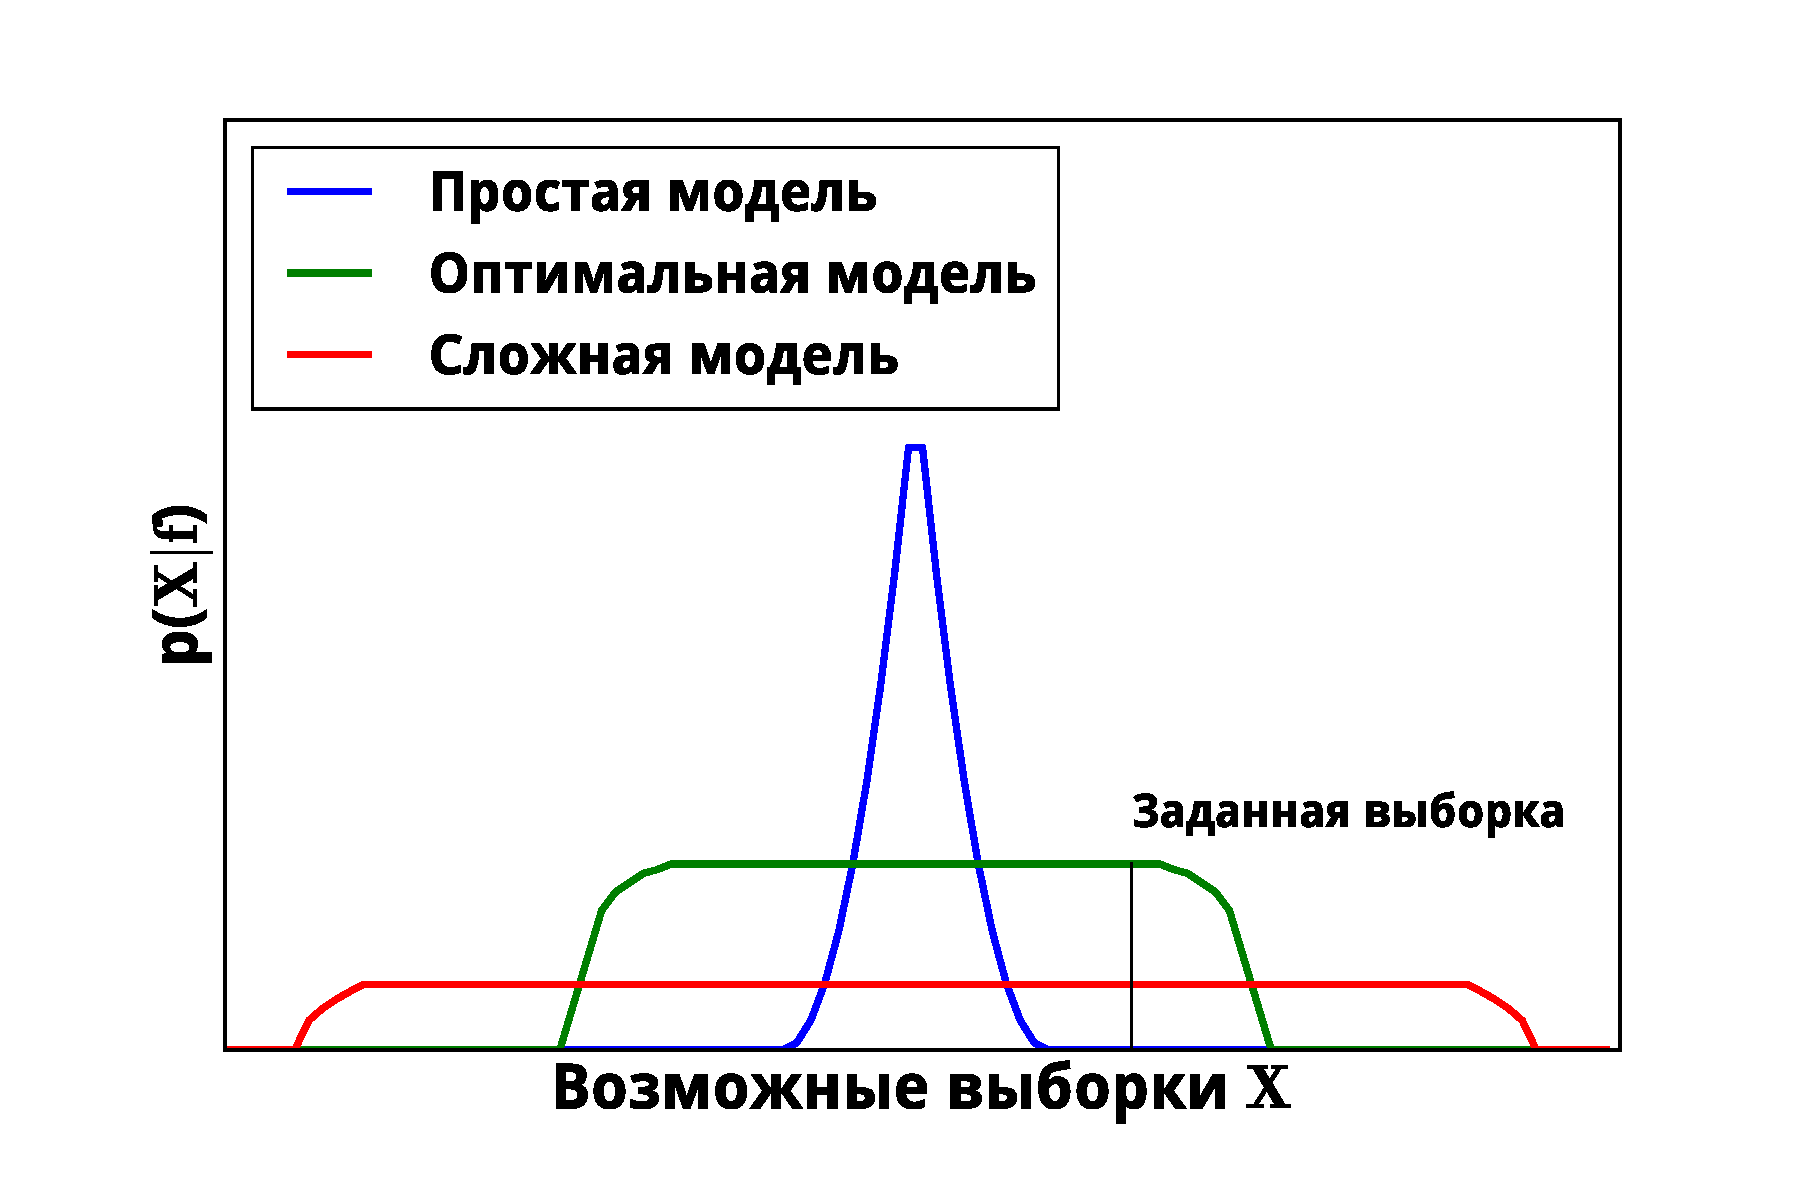
\includegraphics[width=0.35\textwidth]{slide_plots/evidence.pdf}} 
 \subfloat[Аппроксимация выборки полиномами]{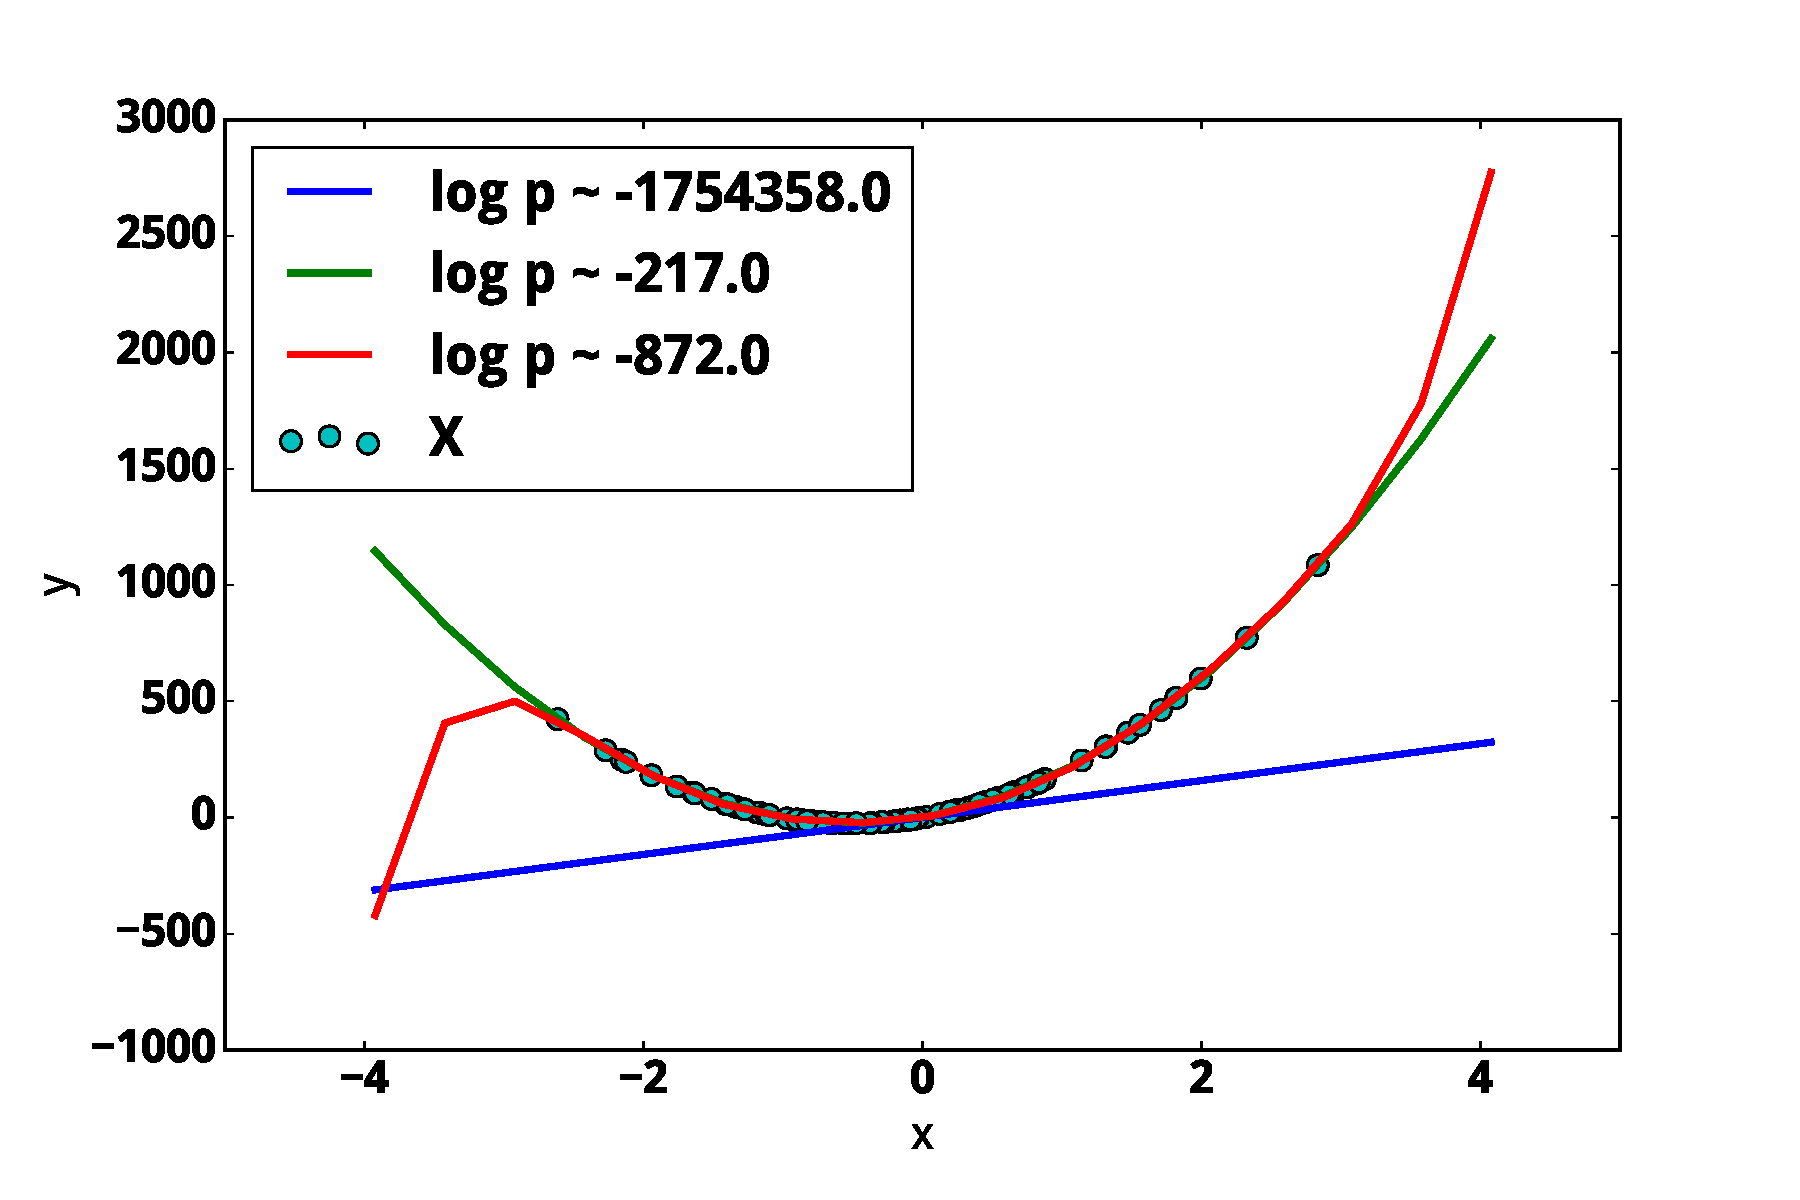
\includegraphics[width=0.35\textwidth]{slide_plots/example.pdf}}

\end{figure}
\end{frame}





\begin{frame}{Выбор оптимальной модели}
\textbf{Основные проблемы выбора оптимальной модели}\\
\begin{itemize}
\item Интеграл правдоподобия $p(\mathbf{y}|\mathbf{X}, \mathbf{h})$  невычислим аналитически.
\item Задача его оптимизации многоэкстремальна и невыпукла.
\end{itemize}
~\\
\textbf{Требуется}\\ 
Предложить метод поиска субоптимального решения задачи оптимизации, обобщающего различные алгоритмы оптимизации:
\begin{itemize}
\item Оптимизация правдоподобия.
\item Последовательное увеличение и снижение сложности модели.
\item Полный перебор вариантов структуры модели.
\end{itemize}

\end{frame}    

                                                                                                              

\begin{frame}{Вариационная нижняя оценка правдоподобия} 
Интеграл правдоподобия невычислим аналитически.\\
\textbf{Правдоподобие модели:}
\[
p(\mathbf{y}|\mathbf{X}) =
 \int_{\mathbf{W}, \boldsymbol{\Gamma} } \textcolor{red}{p(\mathbf{y}|\mathbf{X},\mathbf{W},  \boldsymbol{\Gamma})} \textcolor{blue}{p(\mathbf{W}, \boldsymbol{\Gamma})}d\mathbf{W}d{\boldsymbol{\Gamma}}.                         
\]

Пусть $q(\mathbf{W}, \boldsymbol{\Gamma}) = q_{\mathbf{W}}(\mathbf{W})q_{\boldsymbol{\Gamma}}(\boldsymbol{\Gamma})$ --- непрерывное распределение, аппроксимирующее 
апостериорное распределение $p(\mathbf{W}, \boldsymbol{\Gamma}|\mathbf{y}, \mathbf{X})$.
Получим нижнюю оценку интеграла правдоподобия.\\
$$                                                                                                                                              
        \text{log}~p(\mathbf{y}|\mathbf{X}) \geq 
\textcolor{blue}{\mathsf{E}_q \text{log}~{p(\mathbf{y} | \mathbf{X}, \mathbf{W}, \boldsymbol{\Gamma})}} - \textcolor{red}{\text{D}_{KL}(p(\mathbf{w}, \boldsymbol{\Gamma}) || q(\mathbf{W}, \boldsymbol{\Gamma}))} = \text{log}\hat{{p}}_{q_{\mathbf{W}}q_{\boldsymbol{\Gamma}}}(\mathbf{y}|\mathbf{X}).
$$ 

Полученная оценка совпадает с интегралом правдоподобия при $$D_\text{KL}(q(\mathbf{W}, \boldsymbol{\Gamma})|(p(\mathbf{W}, \boldsymbol{\Gamma}|\mathbf{y}, \mathbf{X}))=0.$$

\end{frame}      

   


\begin{frame}{Общая задача оптимизации}
\begin{block}{Теорема (будет)}
Следующая оптимизационная задача обобщает алгоритмы оптимизации: оптимизация правдоподобия, последовательное увеличение и снижение сложности модели, полный перебор вариантов структуры модели:
\[
\mathbf{h}^{*} = \argmax_{\mathbf{h}} Q = 
\]
\[
= \textcolor{blue}{c_\text{train}\mathsf{E}_{{q}^{*}} \text{log}~{p(\mathbf{y} | \mathbf{X}, \mathbf{W},\boldsymbol{\Gamma}, \mathbf{h}, c_{\text{prior}})}}
 -\]
\[- \textcolor{red}{c_\text{prior}\text{D}_{KL}(p(\mathbf{w}, \boldsymbol{\Gamma} |\mathbf{h}, c_{\text{temp}}) || q^{*}(\mathbf{W}, \boldsymbol{\Gamma}))} -\]
\[
 - \textcolor{OliveGreen}{c_{\text{comb}}\sum_{p' \in \mathbf{P}} \text{D}_{KL}(\boldsymbol{\Gamma} | p')}, 
\]
где 
\[
{q}^{*} = \argmax_{q} L = 
\textcolor{blue}{\mathsf{E}_q \text{log}~{p(\mathbf{y} | \mathbf{X}, \mathbf{W}, \boldsymbol{\Gamma}, \mathbf{A}^{-1}, c_{\text{temp}})}} -\]\[- \textcolor{red}{c_\text{reg}\text{D}_{KL}(p(\mathbf{w}, \boldsymbol{\Gamma} |\mathbf{A}^{-1}, \mathbf{m}, c_{\text{temp}}) || q(\mathbf{W}), q(\boldsymbol{\Gamma}))}
\]
\end{block}
\end{frame}



\begin{frame}
\small
\frametitle{Нижняя вариационная оценка правдоподобия на основе мультистарта}
$$\text{log}p(\mathbf{y}|\mathbf{X}, \mathbf{h}) \geq \mathsf{E}_{q(\mathbf{W)}}\text{log~}p (\mathbf{y}, \mathbf{W}|\mathbf{X}, \mathbf{h}) - \mathsf{E}_{q_{\mathbf{W}}}(-\text{log}(q_\mathbf{W})).$$

\begin{block}{Теорема [Бахтеев, 2016]}Пусть $L$ --- функция потерь, градиент которой ---  непрерывно-дифференцируемая функция с константой Липшица $C$. \\
Пусть $\boldsymbol{\theta} = [\mathbf{W}^1,\dots,\mathbf{W}^k]$ ---  начальные приближения оптимизации модели, $\beta$ --- шаг градиентного спуска.

Тогда разность энтропий на смежных шагах оптимизации приближается следующим образом:
\small
\[
	\mathsf{E}_{q^{\tau}_{\mathbf{W}}}(-\text{log}(q^{\tau}_\mathbf{W})) -  \mathsf{E}_{q^{\tau-1}_{\mathbf{W}}}(-\text{log}(q^{\tau-1}_\mathbf{W}))  \approx  \frac{1}{k}\sum_{r=1}^k \bigl(\beta Tr[\mathbf{H}(\mathbf{W}^r)] - \beta^2 Tr[\mathbf{H}(\mathbf{W}^r)\mathbf{H}(\mathbf{w}^r)]  \bigr),
\]
где $\mathbf{H}$ --- гессиан функции потерь $L$, $q^{\tau}_\mathbf{W}$ --- распределение $q^{\tau}_\mathbf{W}$ в момент оптимизации $\tau$.
\end{block}
\end{frame}



\begin{frame}
\frametitle{Градиентный спуск как вариационная оценка правдоподобия модели}
Для вычисления правдоподобия был предложен ряд алгоритмов, основанных на стохастическом градиентном спуске.
\footnotesize

\begin{multicols}{2}

\begin{figure}
\vspace*{-0.2cm}
\subfloat{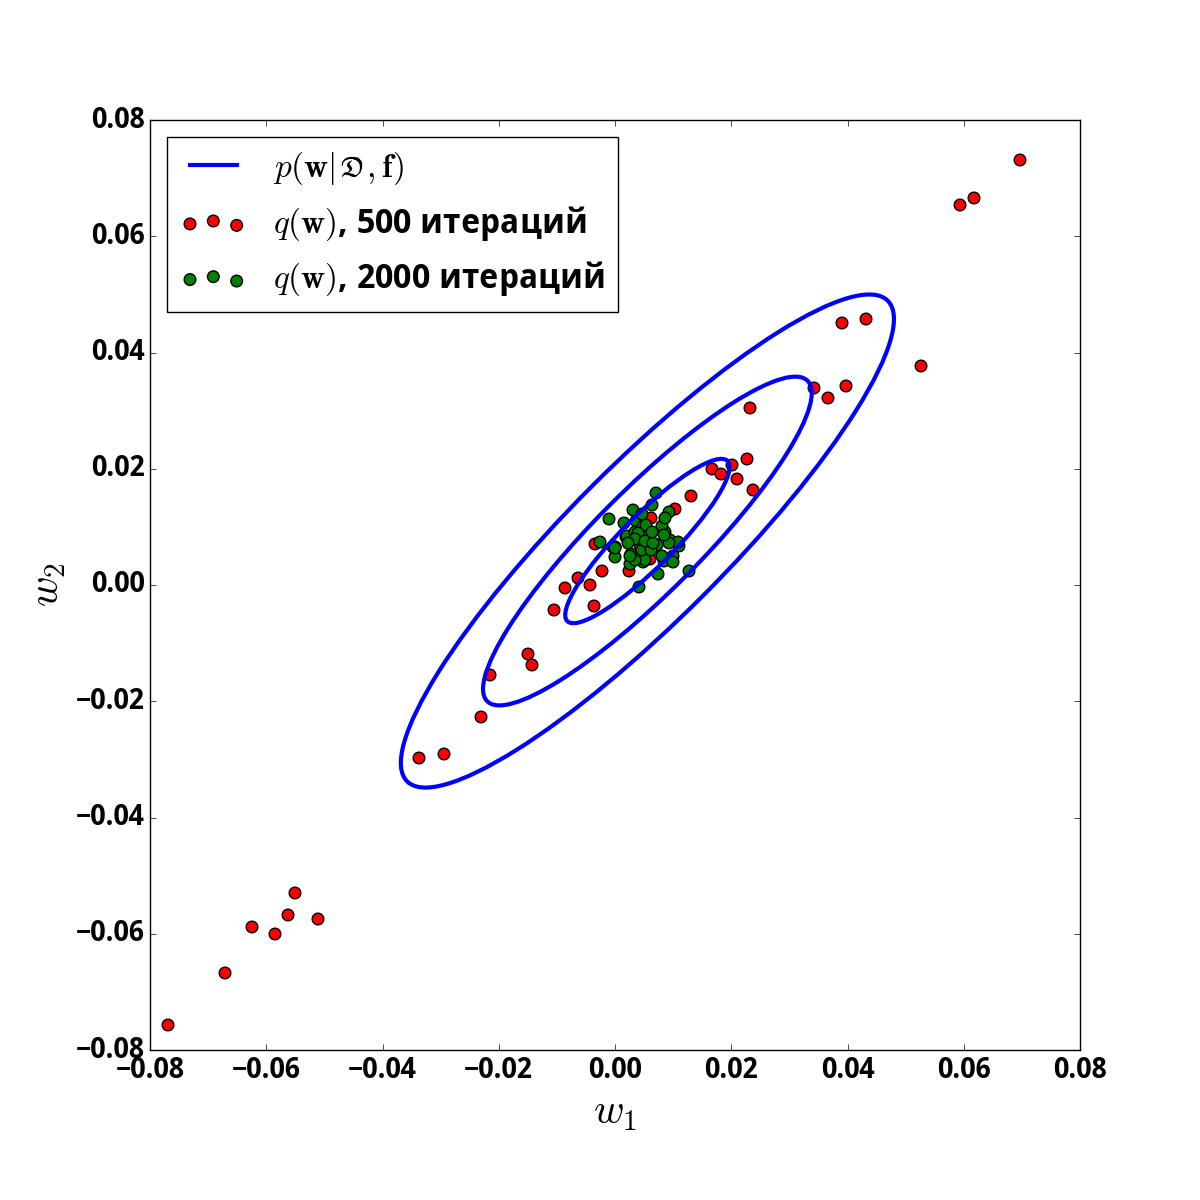
\includegraphics[width=0.52\textwidth]{./slide_plots/sgd_estimate.png}}
\end{figure}

\columnbreak


\begin{figure}
{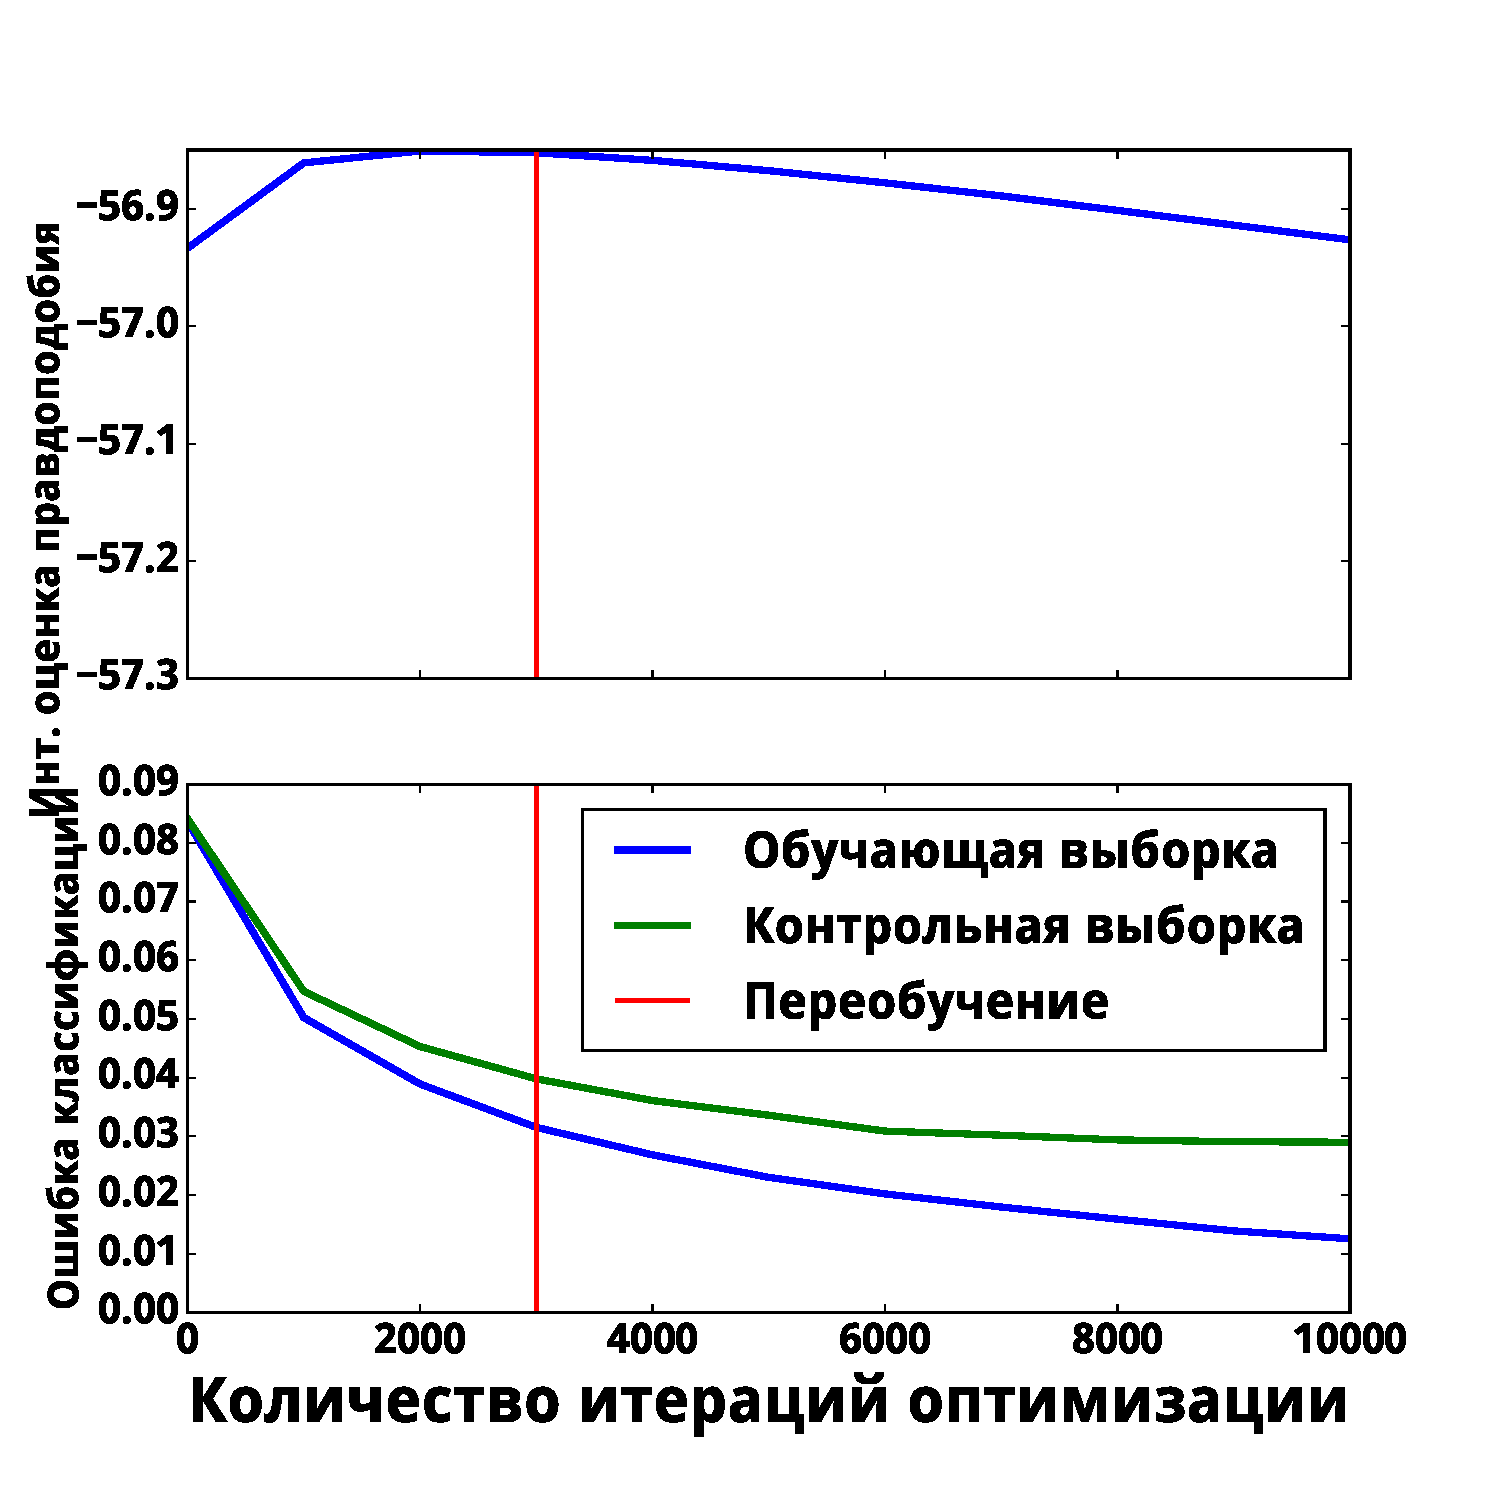
\includegraphics[width=0.52\textwidth]{./slide_plots/sgd_show.pdf}}
\end{figure}
\end{multicols}
\end{frame}



\begin{frame}{Априорное распределение на структуре модели}
\textbf{Распределение Дирихле}\\
\begin{figure}
 \begin{minipage}[t]{.3\textwidth}
        \centering
\begin{tikzpicture}[%
x={(1.7cm,0cm)},
y={(0cm,1.7cm)},
]

\coordinate (A) at (0,0); 
\coordinate (B) at (1,0) ;
\coordinate (C) at (0.5,0.86); 

%Ecken
\node[circle,scale=0.5,fill=black,draw=black](Ap) at (0,0){};
\node[circle,scale=0.5,fill=black,draw=black](Bp) at (1,0){};
\node[circle,scale=0.5,fill=black,draw=black](Cp) at (0.5,0.86){};

%Kanten
\draw[] (A)
-- (B)  node[midway, below]{}
-- (C)      node[midway, right]{}
-- (A)  node[midway, left]{};

\end{tikzpicture}
\caption*{$\tau\to0$}
\end{minipage}
\hfill
 \begin{minipage}[t]{.3\textwidth}
   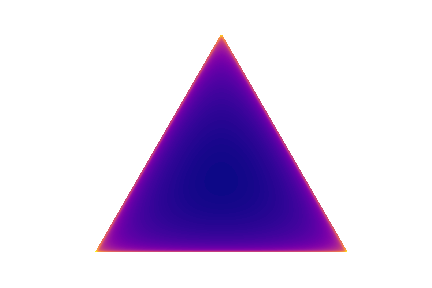
\includegraphics[width=\textwidth]{dir0995.png}
\caption*{$\tau=0.995$}
\end{minipage}
\hfill
 \begin{minipage}[t]{.3\textwidth}
   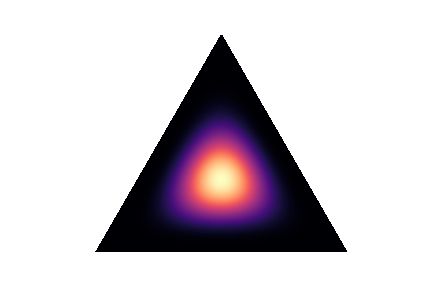
\includegraphics[width=\textwidth]{dir5.png}
\caption*{$\tau=5.0$}
\end{minipage}

\end{figure}

\textbf{Распределение Гумбель-софтмакс}\\
\begin{figure}
 \begin{minipage}[t]{.3\textwidth}
        \centering
\begin{tikzpicture}[%
x={(1.7cm,0cm)},
y={(0cm,1.7cm)},
]

\coordinate (A) at (0,0); 
\coordinate (B) at (1,0) ;
\coordinate (C) at (0.5,0.86); 

%Ecken
\node[circle,scale=0.5,fill=black,draw=black](Ap) at (0,0){};
\node[circle,scale=0.5,fill=black,draw=black](Bp) at (1,0){};
\node[circle,scale=0.5,fill=black,draw=black](Cp) at (0.5,0.86){};

%Kanten
\draw[] (A)
-- (B)  node[midway, below]{}
-- (C)      node[midway, right]{}
-- (A)  node[midway, left]{};

\end{tikzpicture}
\caption*{$\tau\to0$}
\end{minipage}
\hfill
 \begin{minipage}[t]{.3\textwidth}
   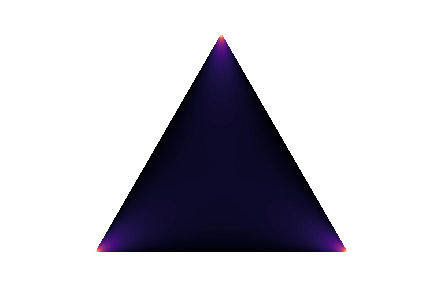
\includegraphics[width=\textwidth]{gs0995.png}
\caption*{$\tau=0.995$}
\end{minipage}
\hfill
 \begin{minipage}[t]{.3\textwidth}
   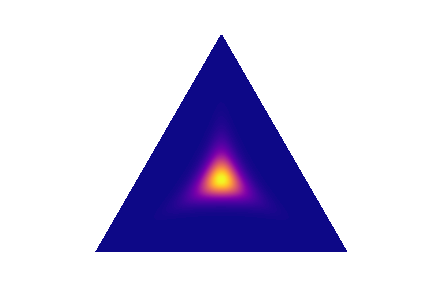
\includegraphics[width=\textwidth]{gs5.png}
\caption*{$\tau=5.0$}
\end{minipage}

\end{figure}
\end{frame}









\begin{frame}{Оператор оптимизации}
\small
\begin{block}{Определение}
Назовем \textit{оператором оптимизации} алгоритм $T$ выбора вектора параметров $\boldsymbol{\theta}'$  по параметрам предыдущего шага $\boldsymbol{\theta}$.
\end{block}
Оператор стохастического градиентного спуска:
\[
	 \hat{\boldsymbol{\theta}} = T \circ T \circ \dots \circ T(\boldsymbol{\theta}_0, \mathbf{A}^{-1}, \mathbf{m}) = T^\eta(\boldsymbol{\theta}_0, \mathbf{A}^{-1}, \mathbf{m}), \quad\text{где}	T(\boldsymbol{\theta}, \mathbf{A}^{-1}, \mathbf{m}) =
\]
\[=\boldsymbol{\theta} - \beta \nabla L(\boldsymbol{\theta}, \mathbf{A}^{-1}, \mathbf{m})|_{\hat{\mathfrak{D}}}, 
\]
$\gamma$ --- длина шага градиентного спуска, $\boldsymbol{\theta}_0$ --- начальное значение параметров $\boldsymbol{\theta}$, $\hat{\mathfrak{D}}$ --- случайная подвыборка исходной выборки $\mathfrak{D}$.


Перепишем итоговую задачу оптимизации:
\[
	{\mathbf{h}}^{*} = \argmax_{\mathbf{h}} Q\left( T^\eta(\boldsymbol{\theta}_0, \mathbf{A}^{-1}, \mathbf{m})\right),
\]
где $\boldsymbol{\theta}_0$ --- начальное значение $\boldsymbol{\theta}$.



\end{frame}




\begin{frame}{Оптимизация гиперпараметров: пример}
\begin{multicols}{2}
\begin{figure}[h]
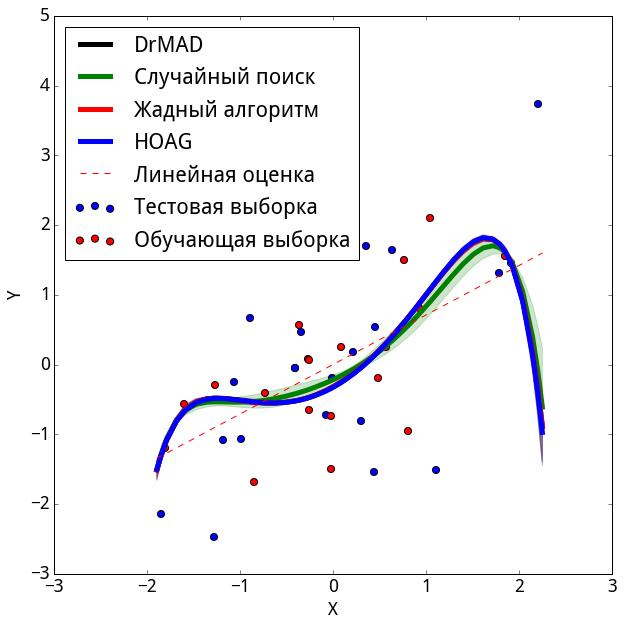
\includegraphics[width=0.4\textwidth]{./slide_plots/poly_cv.png}
\caption*{Кросс-Валидация}
\end{figure}

\begin{figure}[h]
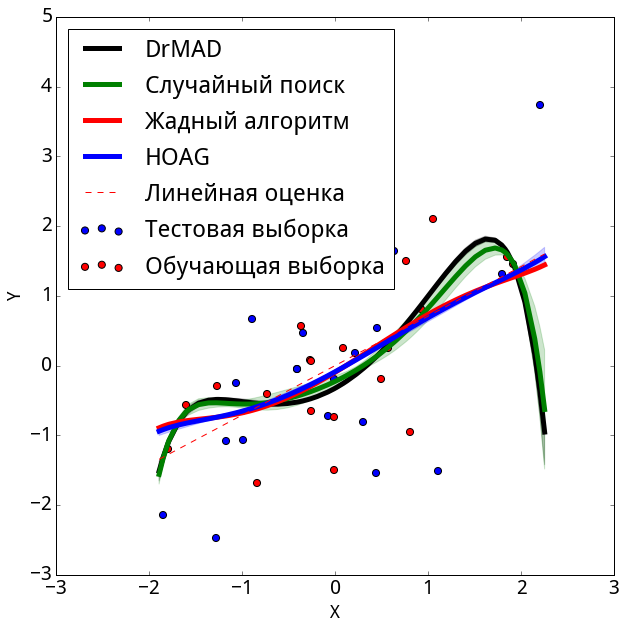
\includegraphics[width=0.4\textwidth]{./slide_plots/poly_var.png}
\caption*{Вариационная оценка}
\end{figure}
\end{multicols}

\end{frame}






\begin{frame}{Оптимизация правдоподобия модели}
\begin{block}{Теорема  [Бахтеев, 2018].}
Пусть существуют параметры распределения $q(\mathbf{W}, \boldsymbol{\Gamma})$, такие что $\text{D}_\text{KL}(q(\mathbf{W}, \boldsymbol{\Gamma})|p(\mathbf{W},  \boldsymbol{\Gamma}| \mathbf{y}, \mathbf{X}, \mathbf{A}, \mathbf{m}, c_\text{temp})) = 0$.\\
Тогда двухуровневая задача оптимизация эквивалентна задаче оптимизации правдоподобия модели:
$$\argmax_{\mathbf{A}, \mathbf{m}}  p(\mathbf{y}|\mathbf{X},\mathbf{A},\mathbf{m}, c_{\text{temp}})$$ 
при $c_{\text{reg}} = c_{\text{prior}} = c_{\text{train}} >0, c_{\text{comb}} = 0$. 
\end{block}
~\\

\end{frame}

\begin{frame}{Параметрическая сложность}
\small
Обозначим за $F(c_{\text{reg}}, c_{\text{train}}, c_{\text{prior}}, c_{\text{comb}}, \mathbf{P}, c_{\text{temp}})$ множество экстремумов функции $L$ при решении задачи двухуровневой оптимизации.
\begin{block}{Теорема [Бахтеев, 2018].}
Пусть $\mathbf{f} \in F(1, 1, c_{\text{prior}}, 0, \varnothing,  c_{\text{temp}} )$.
При устремлении $ c_{\text{prior}}$ к бесконечности параметрическая сложность модели $\mathbf{f}$ устремляется к нулю.
\[
    \lim_{c_{\text{prior}} \to \infty} C_{\text{param}}(\mathbf{f}) = 0.
\]
\end{block}

\begin{block}{Теорема [Бахтеев, 2018].}
Пусть $\mathbf{f}_1 \in F(1, 1, c_{\text{prior}}^1, 0, \varnothing,  c_{\text{temp}} ), \mathbf{f}_2 \in F(1, 1, c_{\text{prior}}^2, 0, \varnothing,  c_{\text{temp}})$, $c_{\text{prior}}^1 < c_{\text{prior}}^2$.\\
Пусть вариационные параметры моделей $\mathbf{f}_1$ и $\mathbf{f}_2$ лежат в области $\mathsf{U}$, в которой соответствующие функции $L$ и $Q$ являются локально-выпуклыми.\\ 
Тогда модель $\mathbf{f}_1$ имеет параметрическую сложность, не меньшую чем у $\mathbf{f}_2$.
\[
    C_\text{param}(\mathbf{f}_1) \geq C_\text{param}(\mathbf{f}_2).
\]
\end{block}


\end{frame}

\begin{frame}{Структурная сложность}
\small

\begin{block}{Теорема  [Бахтеев, 2018].}
Пусть для каждого ребра $(i,j)$ семейства моделей $\mathfrak{F}$ априорное распределение $$p(\boldsymbol{\gamma}_{i,j}) =  \lim_{c_{\text{temp}} \to 0} \mathcal{GS}(c_{\text{temp}}).$$
Пусть $c_{\text{reg}} >0, c_{\text{train}} >0, c_{\text{prior}}>0$.
Пусть $\mathbf{f} \in F(c_{\text{reg}}, c_{\text{train}}, c_{\text{prior}}, 0, \varnothing, c_{\text{temp}})$.
Тогда структурная сложность модели $\mathbf{f}$ равняется нулю.
\[
    C_\text{struct}(\mathbf{f}) = 0.
\]
\end{block}

\begin{block}{Теорема [Бахтеев, 2018].}
Пусть $\mathbf{f}_1 \in F(c_{\text{reg}}, c_{\text{train}},  c_{\text{prior}}, 0, \varnothing,  c^1_{\text{temp}}), \mathbf{f}_2   \in \lim_{c^2_{\text{temp}} \to \infty} F(c_{\text{reg}}, c_{\text{train}},  c_{\text{prior}}, 0, \varnothing,  c^2_{\text{temp}})$.
Пусть вариационные параметры моделей $f_1$ и $f_2$ лежат в области $U$, в которой соответствующие функции $L$ и $Q$ являются локально-выпуклыми. 
Тогда разница структурных сложностей моделей ограничена выражением:
\[
    C_\text{struct}(\mathbf{f}_1)  - C_\text{struct}(\mathbf{f}_2) \leq \textcolor{blue}{\mathsf{E}_q^1 \text{log}~{p(\mathbf{y} | \mathbf{X}, \mathbf{W}, \boldsymbol{\Gamma}. \mathbf{A}^{-1}, c^1_{\text{temp}})}} - \textcolor{blue}{\mathsf{E}_q^2 \text{log}~{p(\mathbf{y} | \mathbf{X}, \mathbf{W}, \boldsymbol{\Gamma}, \mathbf{A}^{-1})}}.
\]
\end{block}

% Схема доказательства:
% расписываем неравенства вида: L_1 - DKL(q_1|p1) <L_2 - DKL(q_2|p1)
% Замечаем, что при стремлении к бесконечности гумбель превращается в равномерное
% выражаем все в равномерном
% замечаем, что D_KL = Entropy + const для равномерного
% все
\end{frame}


\begin{frame}{Полный перебор}
\small
Пусть для каждого ребра $(i,j)$ семейства моделей $\mathfrak{F}$ априорное распределение $$p(\boldsymbol{\gamma}_{i,j}) =  lim_{c_{\text{temp}} \to 0} \mathcal{GS}(c_{\text{temp}}).$$

Рассмотрим последовательность $\mathbf{P}$, состоящую из $N = \prod_{(j,k) \in E} K_{j,k}$ моделей, полученных в ходе оптимизаций вида:
$$f_1 \in F(c_{\text{reg}}, 0, 0, \varnothing, c_{\text{comb}},  c_{\text{temp}}),$$
$$f_2 \in F(c_{\text{reg}}, 0, 0, \{q_1(\boldsymbol{\Gamma})\},  c_{\text{comb}},  c_{\text{temp}}),$$
$$f_3 \in F(c_{\text{reg}}, 0, 0, \{q_1(\boldsymbol{\Gamma}), q_2(\boldsymbol{\Gamma})\},  c_{\text{comb}},  c_{\text{temp}}),$$
где $C_{\text{reg}} > 0,  c_{\text{comb}}>0$.


\begin{block}{Теорема}
Вариационные распределения $q_{\boldsymbol{\Gamma}}$ структур  последовательности $\mathbf{P}$ вырождаются в распределения вида $\delta(\hat{\mathbf{m}})$, где $\hat{\mathbf{m}}$ --- точка на декартовом произведении вершин симплексов структуры модели.

Последовательность соответствует полному перебору структуры $\boldsymbol{\Gamma}$.
\end{block}
\end{frame}


\begin{frame}{Результаты, выносимые на защиту}
\begin{enumerate}
\item Предложен метод выбора модели наиболее правдоподобной структуры, обобщающий ранее описанные алгоритмы оптимизации:
\begin{itemize}
\item оптимизация правдоподобия;
\item последовательное увеличение сложности модели;
\item последовательное снижение сложности модели;
\item полный перебор вариантов структуры модели.
\end{itemize}

\item Предложен алгоритм оптимизации параметров, гиперпараметров и структурных
параметров моделей глубокого обучения.

\item Проведено исследование свойств алгоритмов выбора модели при различных значениях мета-параметров.

\item Проведен вычислительный эксперимент, иллюстрирующий работу предложенного метода.

\end{enumerate}
\end{frame}



\begin{frame}{Список работ автора по теме диссертации}
\tiny
\textbf{Публикации ВАК}
\begin{enumerate}
\item Бахтеев О.Ю., Попова М.С., Стрижов В.В. Системы и средства глубокого обучения в задачах классификации. // Системы и средства информатики. 2016. № 26.2. С. 4-22.
\item Бахтеев О.Ю., Стрижов В.В. Выбор моделей глубокого обучения субоптимальной сложности. // Автоматика и телемеханика. 2018. №8. С. 129-147.
\item Огальцов А.В., Бахтеев О.Ю. Автоматическое извлечение метаданных из научных PDF-документов. // Информатика и её применения. 2018.
\item Смердов А.Н., Бахтеев О.Ю., Стрижов В.В. Выбор оптимальной модели рекуррентной сети в задачах поиска парафраза. // Информатика и ее применения. 2019.
\item Грабовой А.В., Бахтеев О.Ю., Стрижов В.В. Определение релевантности параметров нейросети. // Информатика и её применения. 2019.
\end{enumerate}
\textbf{Выступления с докладом}
\begin{enumerate}
\item ``Восстановление панельной матрицы и ранжирующей модели в разнородных шкалах'', Всероссийская конеренция <<57-я научная конеренция МФТИ>>, 2014.
\item ``A monolingual approach to detection of text reuse in Russian-English collection'', Международная конференция <<Artificial Intelligence and Natural Language Conference>>, 2015.
\item ``Выбор модели глубокого обучения субоптимальной сложности с использованием вариационной оценки правдоподобия'', Международная конференция <<Интеллектуализация обработки информации>>, 2016.
\item ``Author Masking using Sequence-to-Sequence Models'', Международная конференция <<Conference and Labs of the Evaluation Forum>>, 2017.
\item ``Градиентные методы оптимизации гиперпараметров моделей глубокого обучения'', Всероссийская конференция <<Математические методы распознавания образов ММРО>>, 2017.
\item ``Детектирование переводных заимствований в текстах научных статей из журналов, входящих в РИНЦ'', Всероссийская конференция <<Математические методы распознавания образов ММРО>>, 2017.
\item ``Байесовский выбор наиболее правдоподобной структуры модели глубокого обучения'', Международная конференция <<Интеллектуализация обработки информации>>, 2018.
\end{enumerate}
\end{frame}






\end{document}
